\documentclass{beamer}
\usetheme{Zurich}
\usepackage{amsmath, amsfonts, graphicx, multirow}
\title{Neural Networks}
\author{Charlotte Wickham}
\date{\today}

\begin{document}

\frame{\titlepage}

\begin{frame}
	\frametitle{Neural Networks}
	Simplest case
	\begin{itemize}
		\item Have p inputs $\pmb{x}$
		\item Have one hidden layer with each unit being a function ($\phi_j$) of a linear combination of the inputs. 
		\item Each output is a function ($\phi_0$) of a linear combination of the hidden units.
	\end{itemize}
	
	\begin{figure}
	\setkeys{Gin}{width = 0.6\textwidth}
	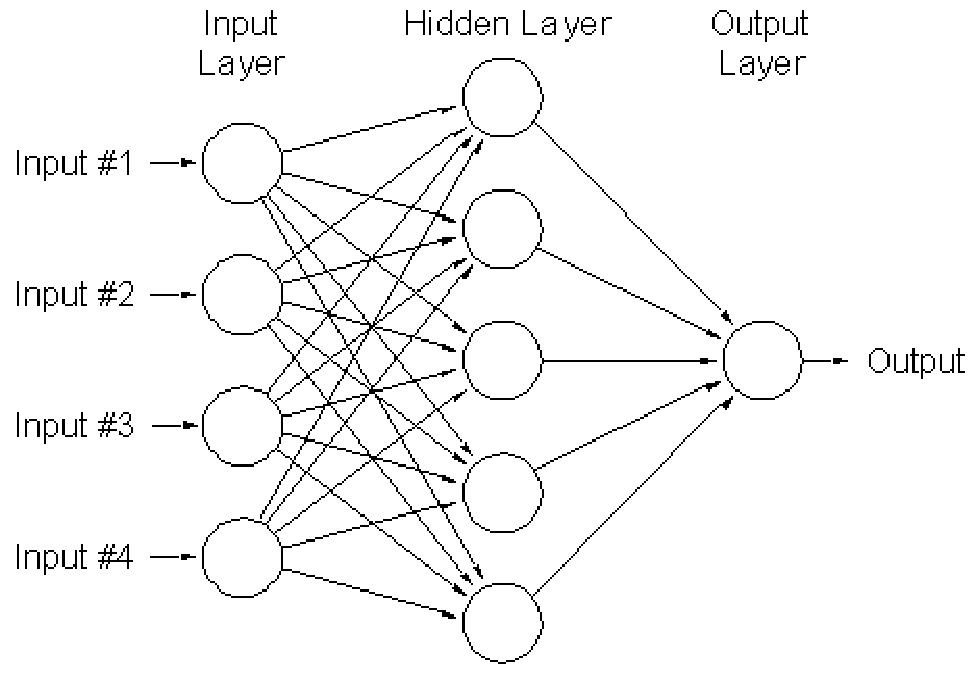
\includegraphics{nnet.pdf}
	\end{figure}
	
\end{frame}

\begin{frame}
	\frametitle{Simplest Case continued}	
	\begin{itemize}
		\item For classification we have $K$ outputs predicting  the probability of belonging to class $k$.
		\item For predicting a single continuous $Y$ we only need one output.
		\item $\phi_j$ is known as the activation function and is often taken to be 
		\[
		\phi_j(v) = \frac{e^v}{1 + e^{v}}
		\]
		\item The output functions $\phi_0$ are often taken as the identity ($\phi_0(t) = t$) for regression, and softmax for K class classification  ($\phi_0(t_k) = e^{t_k} / \sum_k e^{t_k}$).
	\end{itemize}
\end{frame}

\begin{frame}
	\frametitle{General Case}
	\begin{itemize}
		\item Allow more than one layer and connections that skip layers.
		\item 	Also have units with value 1 that feed into all hidden layer and output units to account for constant terms.

		\item 	Then model is:
		\[
		 	y_k = \phi_0\left( \sum_{i \to k }{w_{ik}x_i} + \sum_{j \to k}w_{jk}{\phi_j \Bigl(\sum_{i \to j} w_{ij}x_i \Bigr)} \right)
\]	
		\item Completely parametrized by weight vector $w_{ij}$.
		\item Can be viewed as a very flexible function of the inputs.
	\end{itemize}
\end{frame}

\begin{frame}
	\frametitle{Finding the weights}
	\begin{itemize}
		\item Consider training points $(x_p, t_p)$ and the let the  output of the neural network be $y = f(x; w)$. We want to minimize
		\[
		E(w) =  \sum_p ||t_p - f(x_p; w)||^2
		\]
		or for K class classification (input now $(x_p, t_{p1}, \dots, t_{pk})$, output $y_k = f_k(x; w)$ )
		\[
		E(w) = - \sum_p \sum_k t_{pk} log(f_k(x_p; w)).
		\]
		
		\item Then just a minimization problem.  Many algorithms designed to do this. All iterative.
		\item Need starting points.
		\item Need stopping rule.
	\end{itemize}	
\end{frame}

\begin{frame}
	\frametitle{}
	\begin{itemize}
		\item Starting weights
		
			Generally use random points near zero.  $w_{ij} \sim$ Uniform on $[-0.7,0.7]$ is common.
		\item Stopping rule
		
		Want to avoid overfitting.  
		\begin{itemize}
			\item Early methods stopped minimization early.
			\item Other option is regularization.  Minimize:
			\[
			E(w) =  \sum_p ||t_p - f(x_p; w)||^2 + \lambda \sum_{ij} w_{ij}
			\]
			instead.
			\item Effect is to shrink weights towards zero.
			\item Choose $\lambda$ using cross validation.
			\item 	Also has the advantage that if you use too many hidden units their weights should be shrunk to zero.
		\end{itemize}
	\end{itemize}
\end{frame}

\begin{frame}
	\frametitle{In practice}
	\begin{itemize}
		\item Scale all variables to have mean 0 variance 1 - to ensure input treated equally in regularization.
		\item Choose decay parameter by cross validation.
		\item Number of hidden units generally doesn't matter as long as it is big enough.
		\item Can be sensitive to initial conditions.  Can average a few instances.
	\end{itemize}
\end{frame}

\begin{frame}[fragile]
	\frametitle{Supernova data}
	\begin{verbatim}
      size decay      fit
 [1,]    5 0.010 4.333333
 [2,]    5 0.050 4.377778
 [3,]    5 0.001 4.600000
 [4,]   10 0.010 4.133333
 [5,]   10 0.050 3.977778
 [6,]   10 0.001 4.411111
 [7,]   15 0.010 4.366667
 [8,]   15 0.050 4.322222
 [9,]   15 0.001 4.388889
[10,]   20 0.010 4.422222
[11,]   20 0.050 4.433333
[12,]   20 0.001 4.511111
\end{verbatim}
Fit neural net with 10 hidden units and decay 0.05.  Repeat five times and average result.
\end{frame}

\begin{frame}
	\frametitle{Supernova data}
\begin{itemize}
	\item Disagreement between repetitions
	\begin{table}
	\begin{tabular}{cr|rr}
	& & \multicolumn{2}{c}{NN 1}\\
	& & Other & Supernova\\
	\hline
	\multirow{2}{*}{\rotatebox{90}{NN 2}} & Other &  495 &  15\\
	& Supernova & 10 &  480\\
	\end{tabular}
	\end{table}
	2.5\% disagreement
	\item Prediction error
	\begin{table}
	\begin{tabular}{cr|rr}
	& & \multicolumn{2}{c}{Prediction}\\
	& & Other & Supernova\\
	\hline
	\multirow{2}{*}{\rotatebox{90}{Actual}} & Other &  477 &  23\\
	& Supernova & 28 &  472\\
	\end{tabular}
	\end{table}
		5.1\% error
\end{itemize}

\end{frame}



\end{document}